\section{シャフトに表面トラクション荷重}
この例では、短い円形のシャフトに表面トラクション荷重をかけて曲げを発生させます。その寸法は:
\begin{itemize}
\item 直径:50 mm
\item 長さ: 200 mm
\end{itemize}
\begin{enumerate}
\item 
{[}mm, ton, s,  °C{]}単位の新規ファイルを作成し、ステップ形式のジオメトリをPrePoMaxにインポートします。
次に、パーツをメッシュ分割します。
ここでは、最大要素サイズとして4mmを選択し、その他の設定は変更しませんでした(図\ref{fig:02-01})。
	\begin{figure}[H]
	\centering
	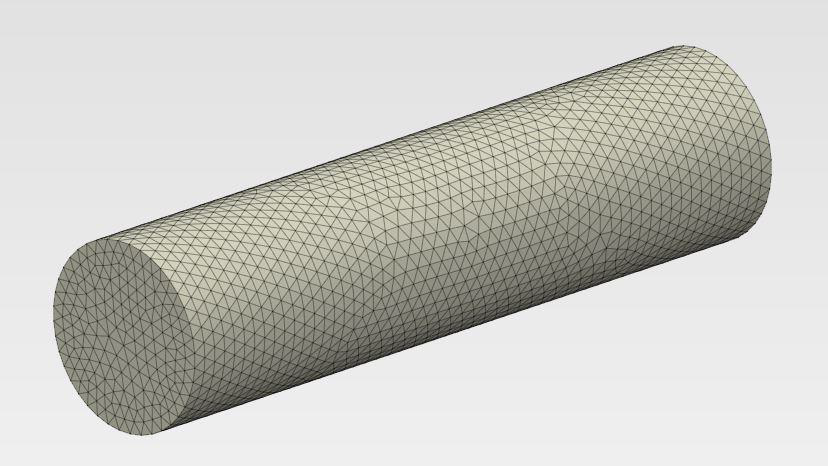
\includegraphics[width=100mm]{fig/02-01.png}
	\caption{シャフト - メッシュ}
	\label{fig:02-01}
	\end{figure}
\item
  新しい材料を定義し、弾性挙動を加え、ヤング率を210000MPa、ポアソン比を0.3と指定します。
  先に作成した材料を参照して新しいソリッドセクションを作成し、そのセクションがこのパーツに割り当てられるようにシャフトを選択します。
\item
  デフォルトの設定で静的解析ステップを定義します。
  固定境界条件をシャフトの片方の端に、表面トラクション荷重を、もう片方の端に割り当てます。
  シャフトの軸に垂直な方向に-500Nの値を指定します(図\ref{fig:02-02})。
	\begin{figure}[H]
	\centering
	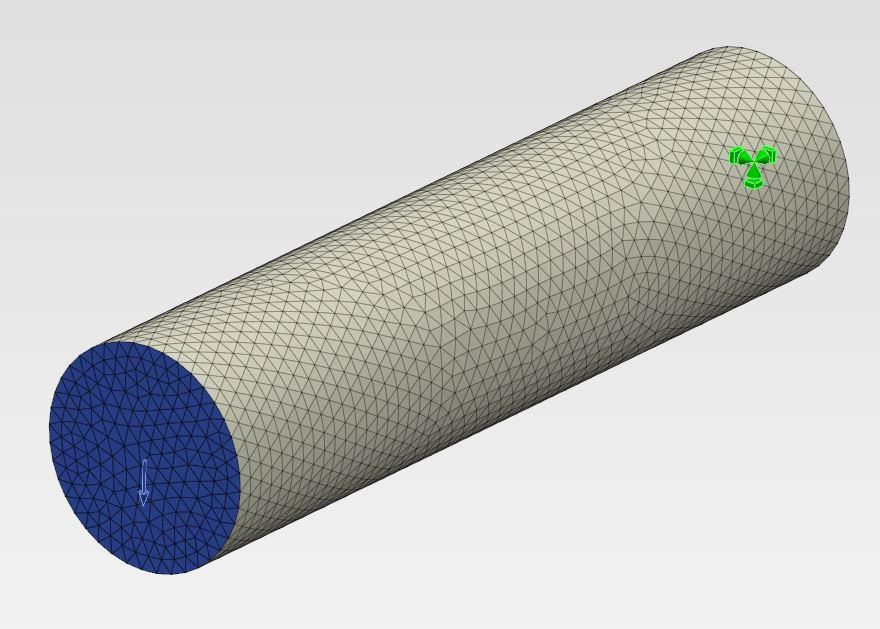
\includegraphics[width=97mm]{fig/02-02.png}
	\caption{シャフト - 境界条件と荷重}
	\label{fig:02-02}
	\end{figure}
\item
  解析を実行し、解析が完了したら結果を開きます。
  変形のスケール係数を400に変更し、非変形モデルを描画するオプションをオンにします。
  変位のコンタープロットを調べ、非変形モデルの形状を隠し、ミーゼス応力のプロットを確認します(図\ref{fig:02-03})。
  分析的に計算された最大応力は8.17MPaで、解析結果を確認しても同様の値が得られます。
	\begin{figure}[H]
	\centering
	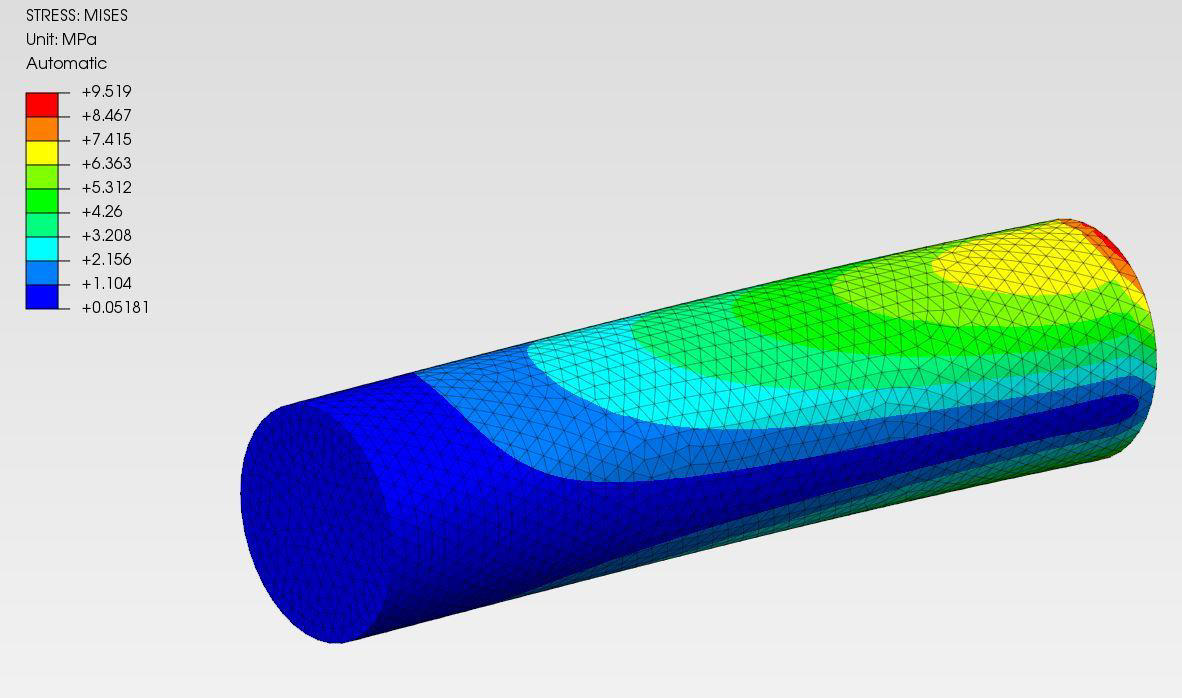
\includegraphics[width=123mm]{fig/02-03.png}
	\caption{シャフト - フォンミーゼス応力}
	\label{fig:02-03}
	\end{figure}
\end{enumerate}